\section[等效原理]{\makebox[5em][s]{等效原理}}\label{sec:12.04}

牛顿力学中,真实力和惯性力是完全不同的。马赫的观点是
几何性的惯性力,实质上也是一种真实的力。爱因斯坦对引力的
研究则认为,在牛顿力学中作为真实力的引力,实质上也就是一
种几何性的力。现在我们简单地介绍一下爱因斯坦的基本观点。

首先,假定在某一空间范围中有恒定的引力,即各处的引力
% 369.jpg
加速度都是$ g $。例如,在地球表面附近,就近似属于这种情况。
如果只有引力,那么,根据式\eqref{eqn:04.06.07}

\begin{equation*}
  \frac { m _ \text{惯} } { m _ \text{引} } = \text{普适常数} = 1
\end{equation*}

所有物体在这个区域中的加速度都完全相同。因此,只要变换到
一个新的参考系$ K' $,$ K' $相对于$ K $系(即原来地球表面附近)的加
速度为$ g $,则一切引力效应都被消除了。任何上述物体的运动都
没有加速度了。

很容易用公式来表达。在参考系$ K $中,牛顿定律是
\begin{equation*}
  m \vec{a} = m \vec{g} + \vec{f} _ \text{外}
\end{equation*}
其中$ \vec{f} _ \text{外} $外表示除引力之外的其他力。对于参考系$ K' $来说,加速度
$ \vec{a} ^ { \prime } = \vec{a} - \vec{g} $,而其他作用力同前,故有
\begin{equation*}
  m \left( \vec{a} ^ { \prime } + \vec{g} \right) = m \vec{g} + \vec{f} _ \text{外}
\end{equation*}
\begin{align*}
  \beforetext{即} m \vec{a} ^ { \prime } = \vec{f} _ \text{外}
\end{align*}
在这个方程中引力不再出现。

现在,参考系$ K' $是引力作用下的自由下落参考系。因此,
由$ m _ \text{惯} / m _ \text{引} $的普适性得出的结论是,在引力的自由下落实验室里,
一切力学现象就如同在一个没有引力的惯性系中是一样的。用这
个局部范围中的力学现象,我们无法区分引力与惯性力。

接着,爱因斯坦作了更进一步的引伸,他认为,在$ K' $系中,
不仅一切力学现象就如同在一个没有引力的惯性系中是一样的,
而且一切物理现象也是一样的。即在局部范围中,用任何物理现
象,我们都无法区分引力与惯性力。

总之,在任何局部范围内,我们总可以找到一种参考系,其
中引力不再存在,就如同总可以找到一种参考系,其中惯性力不
存在一样。引力的本性就在于引力能在某种参考系中被消除。这
就是通常所说的\CJKunderdot{等效原理},它是有关引力的最基本的原理。

等效原理说明引力具有几何性,或“虚拟”性,它的存在与
否,决定于参考系的选择。这种性质,物
理学中其他的力并不具有。例
% 370.jpg
\begin{wrapfigure}[16]{r}{10em}
  \centering
  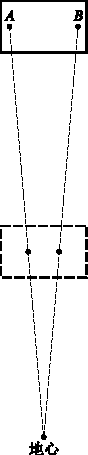
\includegraphics{figure/fig12.13}
  \caption{引力的非均匀性}
  \label{fig:12.13}
\end{wrapfigure}
如,我们不
可能依靠选择参考系而把电磁作用全部消
受掉。引力作用下质点运动的几何性,我
们曾专门在第四章中讨论过(见第四章第
六节)。


在上述的讨论中,我们一再使用“局
部范围”一词。这是因为,实际的引力不
可能是处处均匀的。例如,地球附近的引
力都指向地心,在地球表面上,不同点的
引力的方向是不相同的。引力的大小也随
着与地心的距离变化而变化。对于一个刚
性的自由下落实验室来说,只有在它的质
心那一点上才处于自由下落状态,其余部
分严格说来都不处在自由下落状态。如图
\ref{fig:12.13},在地面附近的自由下落的实验室
中,有两个质点$ A $与$ B $,它们的引力加速度都指向地球中心,所
以二者不平行,相互之间有相对加速度。这样的相对加速度,是
不能通过坐标变换来消除的。因此,原则上说,只有在一个点状
的自由下落体系中才能完全消除引力。这就是必须强调“局部范
围”的原因。
